\documentclass[12pt, a4paper, UTF8]{ctexart}
\usepackage{geometry}
\usepackage{graphicx}
\usepackage{amsmath}
\usepackage{amssymb}
\usepackage{booktabs}
\usepackage{float}
\usepackage{hyperref}
\usepackage{listings}
\usepackage{xcolor}
\usepackage{subfigure}
\usepackage{array}
\usepackage{caption}
\usepackage{tikz}
\usetikzlibrary{positioning, arrows.meta, shapes.geometric}
\graphicspath{{E:/dlhomework/report/}{E:/dlhomework/report/picture/}}

% 基础格式设置
\geometry{left=2.5cm, right=2.5cm, top=2.5cm, bottom=2.5cm}
\hypersetup{colorlinks=true, linkcolor=blue, citecolor=blue, urlcolor=blue}

\lstset{
    language=Python,
    basicstyle=\ttfamily\small,
    keywordstyle=\color{blue!70!black},
    commentstyle=\color{green!40!black},
    stringstyle=\color{red!60!black},
    showstringspaces=false,
    breaklines=true,
    frame=single,
    captionpos=t,
    numbers=left,
    numberstyle=\tiny\color{gray},
    tabsize=4
}

\title{\bfseries 基于GAN的人头图像生成与风格迁移\\
\large 课程大作业报告}
\author{
    组员1：杜锦涛 \quad 学号：524030910186\\
    组员2：曹旭辰 \quad 学号：524030910185\\
}
\date{}

\begin{document}

\maketitle

\begin{abstract}
生成对抗网络（Generative Adversarial Networks, GAN）为无显式概率建模条件下的高维视觉数据生成提供了有效框架。本文围绕人头图像生成与跨域风格迁移两个任务，分别实现并分析了基于深度卷积生成对抗网络（DCGAN）的人脸图像生成模型，以及基于 CycleGAN 的真人头像到动漫头像无配对风格迁移模型。具体而言，我们基于 PyTorch 构建了单卡 GPU 训练的 DCGAN 系统，支持 $64\times64$ 与 $128\times128$ 两种输出分辨率，并在 CelebA 人脸数据集上开展训练、采样、潜空间线性插值以及定量评估；同时，基于标准 \texttt{trainA/trainB/testA/testB} 数据组织实现 CycleGAN，在 $256\times256$ 分辨率下完成真人头像与动漫头像之间的双向映射。针对评估环节，DCGAN 结合 Fr\'echet Inception Distance（FID）与 Inception Score（IS）分析生成样本的分布逼近能力和可辨识性；CycleGAN 则采用双向 FID 与循环重建误差衡量目标域对齐程度和内容保持能力。实验结果表明，DCGAN 能够生成具有基本人脸结构且潜空间连续性较好的低分辨率样本；CycleGAN 能够实现基础的人像到动漫风格迁移，但在反向映射质量、细节保真度以及双向性能平衡方面仍存在进一步优化空间。

\textbf{关键词：}生成对抗网络；DCGAN；CycleGAN；人脸图像生成；风格迁移；FID
\end{abstract}

\tableofcontents

\section{引言}

随着深度生成模型的快速发展，如何从随机潜变量中合成具有真实感、结构一致性和视觉可辨识性的人脸图像，已经成为计算机视觉与图像生成领域的重要研究问题之一。与传统基于显式概率分布估计的方法相比，GAN 通过生成器与判别器之间的对抗博弈实现数据分布拟合，在高维视觉数据生成中表现出较强的表达能力\cite{goodfellow2014gan}。在人脸图像场景中，GAN 不仅能够用于高质量图像采样，还可用于潜空间插值、图像编辑、风格迁移以及数据增强等任务，因此具有较高的研究价值与应用潜力。

在众多 GAN 变体中，DCGAN 是最具代表性的卷积式生成对抗网络之一\cite{radford2015dcgan}。该模型通过在生成器和判别器中引入卷积/反卷积结构、批归一化与稳定激活函数，显著提升了原始 GAN 在图像任务中的训练稳定性与生成质量。尽管 DCGAN 的结构相对经典，但其网络设计、训练流程和潜空间组织方式对理解现代图像生成模型仍然具有基础性意义。

我们围绕 DCGAN 与 CycleGAN 两条技术路线展开实现与分析。对于 DCGAN，研究重点包括：构建与当前代码实现一致的人脸图像生成系统，分析不同分辨率配置下生成器与判别器的结构设计，并通过潜空间插值与 FID/IS 评价生成结果。对于 CycleGAN，研究重点包括：在无配对真人头像与动漫头像数据之间建立双向映射，分析循环一致性与身份映射约束在风格迁移中的作用，并结合测试集可视化结果与双向 FID、循环重建误差评价迁移质量。与标准示例程序相比，当前实现进一步加入了单卡 GPU 约束、固定随机种子控制、显式的训练/评估集分离、按 checkpoint 保存与加载模型、以及面向实验分析的独立采样与评估脚本，因此报告中的模型分析与实验设置均以当前工程实现为准。

\section{相关理论基础}
\subsection{GAN基本原理}

GAN 由生成器 $G$ 与判别器 $D$ 两部分构成。生成器接收潜变量 $z\sim p_z(z)$，将其映射为伪样本 $G(z)$；判别器接收真实样本 $x\sim p_{data}(x)$ 或伪样本 $G(z)$，输出该样本来自真实数据分布的概率。两者通过对抗过程共同优化，其经典极小极大目标函数为
\begin{equation}
\min_G \max_D V(D, G) =
\mathbb{E}_{x \sim p_{data}(x)}[\log D(x)] +
\mathbb{E}_{z \sim p_z(z)}[\log (1 - D(G(z)))].
\end{equation}

上述过程的直观含义在于：判别器希望尽可能准确地区分真实样本与生成样本，而生成器则希望“欺骗”判别器，使伪样本在统计意义上逼近真实数据分布。当训练达到理想平衡时，生成分布 $p_g$ 将逼近真实分布 $p_{data}$，判别器对真实与伪造样本的区分能力下降到随机猜测水平。

尽管 GAN 在视觉生成任务中表现突出，但其训练过程也面临梯度不稳定、模式崩塌（mode collapse）以及收敛难以判断等问题。尤其在高维图像生成任务中，如果网络结构设计不合理，生成器容易产生模糊图像或局部伪影，判别器也可能过强而导致生成器难以获得有效梯度。因此，后续研究普遍从网络结构、归一化方式、损失函数以及优化策略等方面提升 GAN 的训练稳定性。

\subsection{DCGAN模型简介}

DCGAN 的核心思想是在 GAN 框架下系统性引入卷积神经网络结构，从而更适配图像数据的局部空间相关性\cite{radford2015dcgan}。相较于早期使用全连接层的生成对抗网络，DCGAN 具有以下几个关键特征：
\begin{enumerate}
    \item 生成器采用多层转置卷积（ConvTranspose2d）逐步上采样，将低维潜变量映射为高分辨率图像；
    \item 判别器采用多层卷积逐步下采样，将输入图像压缩到真假判别结果；
    \item 中间层引入批归一化（BatchNorm），以缓解训练中的内部协变量偏移；
    \item 生成器使用 ReLU 激活函数，输出层使用 Tanh；判别器使用 LeakyReLU 激活函数；
    \item 网络尽量避免显式全连接主干，以保留卷积结构在图像建模中的归纳偏置。
\end{enumerate}

当前项目中的 DCGAN 实现沿用了上述设计原则，并在工程上进行了两点扩展。其一，生成器和判别器根据参数 \verb|--imageSize| 支持 $64\times64$ 与 $128\times128$ 两种结构配置；其二，训练脚本仅支持单卡 GPU，固定使用 \verb|cuda:0| 进行训练与评估。对于 CelebA 数据集，代码采用平铺目录读取方式，并基于随机种子将完整数据集固定划分为 $90\%$ 训练集与 $10\%$ 评估集，使训练与评估流程可重复且彼此分离。

\subsection{CycleGAN模型简介}

CycleGAN 面向无配对图像到图像翻译任务，其基本思想是在两个域 $X$ 与 $Y$ 之间同时学习正向映射 $G_{AB}: X \rightarrow Y$ 和反向映射 $G_{BA}: Y \rightarrow X$，并分别配置判别器 $D_A$ 与 $D_B$ 用于约束生成样本在目标域上的真实性\cite{zhu2017cyclegan}。与需要严格配对样本的监督式图像翻译方法不同，CycleGAN 仅要求两个域各自具有足量样本，而不要求样本间一一对应，因此更适合真人头像与动漫头像这类难以精确配对的数据场景。

CycleGAN 的核心约束包括三类。第一，对抗损失保证 $G_{AB}(x)$ 在统计上接近域 $Y$，且 $G_{BA}(y)$ 接近域 $X$；第二，循环一致性损失要求 $x \rightarrow G_{AB}(x) \rightarrow G_{BA}(G_{AB}(x))$ 能尽量回到原始输入，抑制内容结构崩塌；第三，身份映射损失要求已经属于目标域的样本通过对应生成器后尽量保持不变，从而减弱过度着色和风格漂移。当前项目中的实现使用基于残差块的生成器、PatchGAN 判别器、最小二乘对抗损失以及全测试集双向 FID 评估，构成了较为完整的无配对风格迁移实验框架。

\subsection{评估指标（FID与IS）}

为了更全面地评估生成模型的性能，我们在 DCGAN 实验中采用 FID 与 IS 两类常用指标。两者均基于预训练 InceptionV3 网络提取的深层语义特征，但关注点并不相同。

\paragraph{(1) Fr\'echet Inception Distance (FID).}
FID 用于衡量生成样本分布与真实样本分布之间的距离\cite{heusel2017fid}。设真实样本特征服从高斯分布 $\mathcal{N}(\mu_r, \Sigma_r)$，生成样本特征服从高斯分布 $\mathcal{N}(\mu_g, \Sigma_g)$，则 FID 定义为
\begin{equation}
\mathrm{FID} = \|\mu_r - \mu_g\|_2^2 +
\mathrm{Tr}\left(\Sigma_r + \Sigma_g - 2(\Sigma_r \Sigma_g)^{1/2}\right).
\end{equation}
FID 越低，说明生成样本在高层语义分布上越接近真实样本。相较于仅考察单样本分类置信度的指标，FID 对模式多样性与分布匹配更敏感，因此在生成任务中具有较高参考价值。

\paragraph{(2) Inception Score (IS).}
IS 用于衡量生成图像的类别可辨识性与整体多样性\cite{salimans2016improved}。其基本思想是：一方面，单张图像的条件类别分布 $p(y|x)$ 应尽量尖锐，即图像应当清晰且可识别；另一方面，整体边缘分布 $p(y)$ 应尽量均匀，即生成结果应具有较好的多样性。其形式可表示为
\begin{equation}
\mathrm{IS} = \exp\left(
\mathbb{E}_{x}\left[
\mathrm{KL}\big(p(y|x)\,\|\,p(y)\big)
\right]
\right).
\end{equation}
IS 越高，通常意味着生成结果越清晰且类别覆盖更广。但由于 IS 不直接比较真实分布与生成分布之间的距离，因此在实际使用中常与 FID 结合分析。

在当前代码实现中，评估器基于 InceptionV3 的中间特征提取模块进行计算，并按照训练 epoch 保存 FID/IS 历史记录、柱状图以及 CSV 文件。由此，实验分析不仅可以比较最终结果，还可以观察训练过程中生成分布逐步逼近真实分布的趋势。

\section{基于DCGAN的人脸图像生成}
\subsection{模型结构}

我们采用的 DCGAN 模型结构由生成器与判别器两部分组成，具体实现见项目代码中的 \verb|dcgan_model.py|。模型的一个特点是结构由参数 \verb|imageSize| 控制，可在 $64\times64$ 与 $128\times128$ 两个分辨率上切换，而不改变训练主循环逻辑。

\begin{figure}[H]
\centering
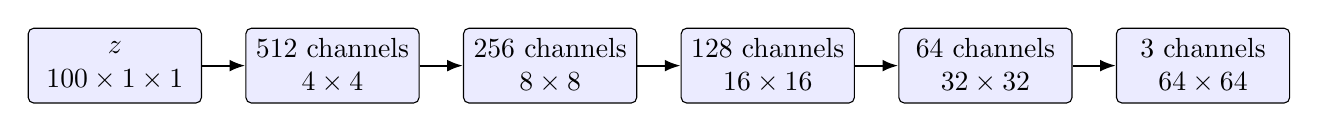
\begin{tikzpicture}[
    node distance=0.55cm,
    box/.style={draw, rounded corners=2pt, minimum height=0.95cm, minimum width=2.2cm, align=center, fill=blue!8},
    arrow/.style={-{Latex[length=2mm]}, thick}
]
\node[box] (z) {$z$\\$100\times1\times1$};
\node[box, right=of z] (g1) {$512$ channels\\$4\times4$};
\node[box, right=of g1] (g2) {$256$ channels\\$8\times8$};
\node[box, right=of g2] (g3) {$128$ channels\\$16\times16$};
\node[box, right=of g3] (g4) {$64$ channels\\$32\times32$};
\node[box, right=of g4] (g5) {$3$ channels\\$64\times64$};
\draw[arrow] (z) -- (g1);
\draw[arrow] (g1) -- (g2);
\draw[arrow] (g2) -- (g3);
\draw[arrow] (g3) -- (g4);
\draw[arrow] (g4) -- (g5);
\end{tikzpicture}
\caption{当前实现中 $64\times64$ 生成器的分辨率与通道演化示意图。若设置 \texttt{imageSize=128}，则在末端额外增加一层上采样，将 $32\times32$ 经 $64\times64$ 过渡到 $128\times128$。}
\end{figure}

\begin{figure}[H]
\centering
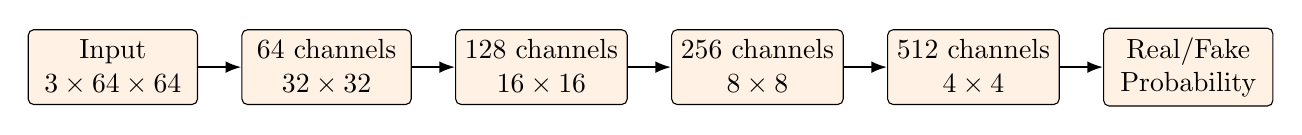
\begin{tikzpicture}[
    node distance=0.55cm,
    box/.style={draw, rounded corners=2pt, minimum height=0.95cm, minimum width=2.15cm, align=center, fill=orange!10},
    arrow/.style={-{Latex[length=2mm]}, thick}
]
\node[box] (x) {Input\\$3\times64\times64$};
\node[box, right=of x] (d1) {$64$ channels\\$32\times32$};
\node[box, right=of d1] (d2) {$128$ channels\\$16\times16$};
\node[box, right=of d2] (d3) {$256$ channels\\$8\times8$};
\node[box, right=of d3] (d4) {$512$ channels\\$4\times4$};
\node[box, right=of d4] (out) {Real/Fake\\Probability};
\draw[arrow] (x) -- (d1);
\draw[arrow] (d1) -- (d2);
\draw[arrow] (d2) -- (d3);
\draw[arrow] (d3) -- (d4);
\draw[arrow] (d4) -- (out);
\end{tikzpicture}
\caption{当前实现中 $64\times64$ 判别器结构示意图。若设置 \texttt{imageSize=128}，则在输入端增加一层下采样，以适配更高分辨率输入。}
\end{figure}

\subsubsection{生成器}

生成器的输入为服从标准高斯分布的潜变量 $z\in\mathbb{R}^{100}$，其张量形状为 $(100,1,1)$。在默认配置 \verb|ngf=64| 下，$64\times64$ 生成器通过五层转置卷积逐步完成空间尺寸扩展，通道数按 $512 \rightarrow 256 \rightarrow 128 \rightarrow 64 \rightarrow 3$ 递减。每个中间卷积块均采用 \verb|BatchNorm2d + ReLU|，输出层采用 \verb|Tanh|，从而将像素值映射到 $[-1,1]$ 范围，与数据预处理中的归一化方式保持一致。

当目标分辨率切换到 $128\times128$ 时，当前实现并未重新设计整个网络，而是在 $64\times64$ 生成器的末端额外增加一层反卷积上采样模块，将特征图继续放大到 $128\times128$。这种设计具有较强的工程可复用性，使训练脚本能够在不改变优化流程的前提下支持不同分辨率的人脸生成实验。

\subsubsection{判别器}

判别器的作用是对输入图像的真实性进行二分类判断。对于 $64\times64$ 配置，判别器采用四层下采样卷积逐步压缩空间分辨率，并最终通过一个单通道卷积与 \verb|Sigmoid| 输出真假概率。在默认配置 \verb|ndf=64| 下，其通道变化路径为 $3 \rightarrow 64 \rightarrow 128 \rightarrow 256 \rightarrow 512 \rightarrow 1$。除第一层外，后续卷积块均配合 \verb|BatchNorm2d| 使用，激活函数采用 \verb|LeakyReLU(0.2)|，以减缓梯度消失问题。

对于 $128\times128$ 输入，判别器在前端增加一层额外卷积，以匹配更高分辨率图像的下采样需求。由此，模型能够在保持判别头结构一致的前提下，适配双分辨率实验设置。

\subsection{损失函数与训练流程}

当前实现采用标准二元交叉熵损失（Binary Cross Entropy, BCE）作为对抗学习目标。判别器优化目标可表示为
\begin{equation}
\mathcal{L}_D = -\mathbb{E}_{x \sim p_{data}(x)}[\log D(x)]
- \mathbb{E}_{z \sim p_z(z)}[\log (1 - D(G(z)))] ,
\end{equation}
生成器优化目标则等价于
\begin{equation}
\mathcal{L}_G = -\mathbb{E}_{z \sim p_z(z)}[\log D(G(z))].
\end{equation}

在实现层面，每个 mini-batch 的训练过程遵循“先更新判别器，再更新生成器”的顺序。具体而言，判别器首先利用真实图像计算 \verb|errD_real|，随后利用由噪声采样生成的伪图像计算 \verb|errD_fake|，二者求和后完成一次参数更新。之后，生成器重新将伪图像送入判别器，并以“将伪样本判为真”为目标计算 \verb|errG|，进而更新生成器参数。优化器方面，生成器与判别器均采用 Adam，学习率设置为 $2\times10^{-4}$，一阶动量参数为 $\beta_1=0.5$。

\begin{figure}[H]
\centering
\resizebox{\textwidth}{!}{
\begin{tikzpicture}[
    node distance=0.28cm,
    box/.style={draw, rounded corners=2pt, minimum height=0.9cm, minimum width=2.0cm, align=center, fill=green!8},
    arrow/.style={-{Latex[length=2mm]}, thick}
]
\node[box] (data) {CelebA 数据读取\\Resize / Crop\\Normalize};
\node[box, right=of data] (split) {固定随机种子\\训练集:评估集\\= 9:1};
\node[box, right=of split] (dstep) {更新判别器\\真实样本\\+ 伪样本};
\node[box, right=of dstep] (gstep) {更新生成器\\最大化伪样本\\真实性};
\node[box, right=of gstep] (eval) {按 \texttt{eval\_freq}\\计算 FID\\与 IS};
\draw[arrow] (data) -- (split);
\draw[arrow] (split) -- (dstep);
\draw[arrow] (dstep) -- (gstep);
\draw[arrow] (gstep) -- (eval);
\end{tikzpicture}
}
\caption{当前 DCGAN 实现的训练与评估流程示意图。}
\end{figure}

除训练主循环外，代码中还引入了两个与实验分析密切相关的机制。其一，训练过程中使用固定噪声 \verb|fixed_noise| 定期生成可视化样本，以便横向比较不同 epoch 下同一批潜变量的输出质量变化；其二，每隔若干 epoch 在独立的评估集上计算一次 FID 与 IS，并将结果保存为柱状图与 CSV，从而形成定性与定量相结合的分析依据。

\section{基于CycleGAN的人脸到动漫风格迁移}
\subsection{模型结构}
\noindent 当前实现中的 CycleGAN 由两个生成器和两个判别器共同组成：生成器 $G_{AB}$ 负责将真人头像映射为动漫头像，生成器 $G_{BA}$ 负责将动漫头像映射回真人头像；判别器 $D_B$ 负责区分真实动漫头像与 $G_{AB}$ 的输出，判别器 $D_A$ 负责区分真实真人头像与 $G_{BA}$ 的输出。整个系统在结构上仍保持经典 CycleGAN 的双向对抗框架，但在工程实现上加入了谱归一化、显式测试集评估等机制，以增强训练稳定性和实验可追踪性。

\subsubsection{生成器}
\noindent 生成器采用基于 Johnson 风格迁移网络的残差结构\cite{johnson2016perceptual}。在当前代码中，输入图像首先经过反射填充和 $7\times7$ 卷积映射到 64 维特征空间，然后通过两层步长为 2 的卷积完成下采样，使空间分辨率从 $256\times256$ 逐步降至 $64\times64$，同时通道数扩展为 256。中间主体由 9 个残差块构成，每个残差块包含两次卷积、实例归一化与 ReLU 激活，并通过跳跃连接学习残差信息。随后，网络通过两次上采样和卷积逐步恢复空间分辨率，并在输出端采用 \verb|Tanh| 将像素归一化到 $[-1,1]$。值得注意的是，当前实现为生成器中的卷积层也加入了谱归一化，这与原始 CycleGAN 并不完全相同，但在本次实验中有助于缓解训练震荡。

\subsubsection{判别器}
\noindent 判别器采用 $70\times70$ PatchGAN 结构。与对整幅图像仅输出单个真假标量不同，PatchGAN 会对输入图像的局部区域分别给出真假判断，从而更强调纹理、边缘和局部风格的真实性。当前实现中，判别器由四个下采样卷积块和一个输出卷积层组成，每个卷积块包含谱归一化卷积、实例归一化与 LeakyReLU 激活，最终输出一个二维响应图。由于每个位置对应输入图像的局部感受野，因此该结构能够在较低参数量下有效约束动漫纹理、眼部描线和头发色块等局部风格特征。

\subsection{损失函数与训练流程}

当前实现并未采用原始 GAN 中常见的二元交叉熵判别损失，而是使用最小二乘对抗损失（Least Squares GAN, LSGAN）形式，即在代码中以 \verb|MSELoss| 实现生成器和判别器的对抗目标。对于真人域 $X$ 与动漫域 $Y$，双向对抗损失可写为
\begin{equation}
\mathcal{L}_{\mathrm{GAN}}(G_{AB}, D_B, X, Y)
= \mathbb{E}_{y \sim p_Y(y)} \left[(D_B(y)-1)^2\right]
+ \mathbb{E}_{x \sim p_X(x)} \left[D_B(G_{AB}(x))^2\right],
\end{equation}
\begin{equation}
\mathcal{L}_{\mathrm{GAN}}(G_{BA}, D_A, Y, X)
= \mathbb{E}_{x \sim p_X(x)} \left[(D_A(x)-1)^2\right]
+ \mathbb{E}_{y \sim p_Y(y)} \left[D_A(G_{BA}(y))^2\right].
\end{equation}

为了保证跨域翻译后的内容仍与输入样本保持一致，CycleGAN 进一步引入循环一致性损失：
\begin{equation}
\mathcal{L}_{\mathrm{cyc}}(G_{AB}, G_{BA})
= \mathbb{E}_{x \sim p_X(x)} \left[\|G_{BA}(G_{AB}(x)) - x\|_1\right]
+ \mathbb{E}_{y \sim p_Y(y)} \left[\|G_{AB}(G_{BA}(y)) - y\|_1\right].
\end{equation}
同时，为了减弱已经处于目标域的样本在映射过程中被过度修改，代码中还加入身份映射损失：
\begin{equation}
\mathcal{L}_{\mathrm{id}}(G_{AB}, G_{BA})
= \mathbb{E}_{x \sim p_X(x)} \left[\|G_{BA}(x) - x\|_1\right]
+ \mathbb{E}_{y \sim p_Y(y)} \left[\|G_{AB}(y) - y\|_1\right].
\end{equation}
最终生成器总损失为
\begin{equation}
\mathcal{L}_G
= \mathcal{L}_{\mathrm{GAN}}
+ \lambda_{\mathrm{cyc}} \mathcal{L}_{\mathrm{cyc}}
+ \lambda_{\mathrm{id}} \mathcal{L}_{\mathrm{id}},
\end{equation}
其中当前实现取 $\lambda_{\mathrm{cyc}}=10.0$，$\lambda_{\mathrm{id}}=5.0$。

在训练流程上，每个 mini-batch 中先更新两个生成器，再分别更新判别器 $D_A$ 和 $D_B$。为了抑制判别器对最新伪样本的过拟合，代码中还引入了 \verb|ReplayBuffer| 保存历史生成结果，并在判别器更新时混合使用近期伪样本和当前伪样本。此外，训练脚本会周期性地从测试集抽取样本，拼接保存 \verb|real_A|、\verb|fake_B|、\verb|recov_A|、\verb|id_A|、\verb|real_B|、\verb|fake_A|、\verb|recov_B| 与 \verb|id_B| 八类图像，用于同步观察风格迁移、循环重建和身份保持三类效果。

\begin{figure}[H]
\centering
\includegraphics[width=0.76\textwidth]{{train process.png}}
\caption{CycleGAN 训练流程示意图。该流程体现了双向生成器、双向判别器以及循环一致性约束共同参与优化的基本机制。}
\label{fig:cyclegan-train-process}
\end{figure}

\section{实验设置}
\subsection{数据集介绍}
\subsubsection{CelebA人脸数据集}

我们的 DCGAN 实验以 CelebA 数据集作为真实人脸数据来源。CelebA 包含大规模人脸图像样本，具有较为统一的对齐方式和丰富的人脸外观变化，适合作为人脸生成模型的训练数据。与许多基于类别子目录的数据集不同，当前实现针对 CelebA 采用平铺目录读取方式，即 \verb|img_align_celeba| 目录下直接存放图像文件而不再划分类别子文件夹。

在数据预处理环节，代码首先对输入图像进行尺寸缩放与中心裁剪，再将像素归一化到 $[-1,1]$ 区间。对于当前 CelebA 实验，脚本基于固定随机种子将整份数据集划分为训练集与评估集，比例为 $9:1$。其中训练集用于模型参数优化，评估集仅用于 FID 与 IS 计算，避免了训练样本与评估样本完全重合带来的分布偏差。

\subsubsection{动漫人脸数据集}

CycleGAN 实验使用的头像风格迁移数据以 \verb|archive| 目录组织，采用标准的无配对图像翻译数据格式，即分别包含 \verb|trainA|、\verb|trainB|、\verb|testA| 和 \verb|testB| 四个子目录。其中，A 域表示真人头像，B 域表示动漫头像；训练阶段使用 \verb|trainA/trainB| 中的无配对样本，评估和可视化阶段使用 \verb|testA/testB| 中的测试样本。根据当前本地数据统计，训练集中 A、B 两个域各包含 3400 张图像，测试集中各包含 100 张图像。

与 DCGAN 中直接从随机潜变量生成图像不同，CycleGAN 的输入是来自源域的真实头像，因此数据预处理策略更强调空间尺度统一与风格翻译一致性。当前实现将输入图像统一缩放到略大于目标分辨率的尺寸后随机裁剪到 $256\times256$，同时在训练阶段执行随机水平翻转，并将像素归一化到 $[-1,1]$ 区间。这一处理方式兼顾了数据增广与尺度对齐，有利于提升风格迁移模型在局部区域上的泛化能力。

\subsection{实验环境与超参数}

\subsubsection{DCGAN}

对应的 DCGAN 实验在单卡 GPU 环境下进行，训练脚本固定使用 \verb|cuda:0|。当 CUDA 不可用时，程序会直接报错退出，而不会退回 CPU 路径，从而保证训练配置与资源使用的一致性。为提高卷积运算效率，代码中启用了 \verb|cudnn.benchmark|。

实验所采用的主要超参数设置如表 \ref{tab:dcgan-hyper} 所示。除非特别说明，潜变量维度设置为 100，批大小设置为 64，训练轮数设置为 25，优化器使用 Adam，学习率为 $2\times10^{-4}$。此外，代码支持通过 \verb|imageSize| 在 $64\times64$ 与 $128\times128$ 间切换，以比较不同生成分辨率对结果质量的影响。

\begin{table}[H]
\centering
\caption{DCGAN 实验的主要超参数设置}
\label{tab:dcgan-hyper}
\begin{tabular}{>{\centering\arraybackslash}m{3.2cm} >{\centering\arraybackslash}m{3cm} m{6cm}}
\toprule
参数 & 取值 & 说明 \\
\midrule
\verb|dataset| & \verb|celeba| & 人脸数据集类型 \\
\verb|imageSize| & 64 / 128 & 输入输出分辨率，同时决定网络结构 \\
\verb|batchSize| & 64 & 每个 mini-batch 的样本数 \\
\verb|nz| & 100 & 潜变量维度 \\
\verb|ngf| & 64 & 生成器通道基数 \\
\verb|ndf| & 64 & 判别器通道基数 \\
\verb|niter| & 25 & 训练 epoch 数 \\
\verb|lr| & 0.0002 & Adam 学习率 \\
\verb|beta1| & 0.5 & Adam 一阶动量参数 \\
\verb|eval\_freq| & 5 & 每隔多少个 epoch 进行一次评估 \\
\verb|fid\_samples| & 5000 & 评估时生成样本数量 \\
\bottomrule
\end{tabular}
\end{table}

\subsubsection{CycleGAN}

对应的 CycleGAN 实验同样在单卡 GPU 环境下完成，模型输入输出分辨率固定为 $256\times256$。训练脚本使用两个 ResNet 生成器和两个 PatchGAN 判别器，并在生成器与判别器的卷积层中引入谱归一化。优化器统一采用 Adam，学习率设置为 $2\times10^{-4}$，动量参数分别为 $\beta_1=0.5$ 和 $\beta_2=0.999$。与 DCGAN 以随机噪声采样为核心不同，CycleGAN 的训练依赖两个域的无配对样本，因此 batch size 固定为 1，以保持细粒度的样本级对抗更新。

实验所采用的主要超参数如表 \ref{tab:cyclegan-hyper} 所示。根据当前实现，学习率在前 100 个 epoch 内保持不变，随后再线性衰减至 0；训练过程中按照设定的 \verb|sample_interval| 保存可视化结果，并通过 \verb|latest| checkpoint 管理最新模型权重。评估阶段直接在整个测试集上计算 \verb|FID_A2B|、\verb|FID_B2A|、\verb|cycle_L1_A| 与 \verb|cycle_L1_B|。

\begin{table}[H]
\centering
\caption{CycleGAN 实验的主要超参数设置}
\label{tab:cyclegan-hyper}
\begin{tabular}{>{\centering\arraybackslash}m{3.2cm} >{\centering\arraybackslash}m{3cm} m{6cm}}
\toprule
参数 & 取值 & 说明 \\
\midrule
\verb|dataset_name| & \verb|archive| & 真人/动漫双域数据集 \\
\verb|img_height| / \verb|img_width| & 256 / 256 & 输入输出分辨率 \\
\verb|batch_size| & 1 & 单样本对抗更新 \\
\verb|n_epochs| & 200 & 总训练轮数 \\
\verb|decay_epoch| & 100 & 开始线性衰减学习率的轮数 \\
\verb|lr| & 0.0002 & Adam 学习率 \\
\verb|b1| / \verb|b2| & 0.5 / 0.999 & Adam 动量参数 \\
\verb|n_residual_blocks| & 9 & 生成器残差块数 \\
\verb|lambda_cyc| & 10.0 & 循环一致性损失权重 \\
\verb|lambda_id| & 5.0 & 身份映射损失权重 \\
\verb|sample_interval| & 100 & 可视化保存间隔（batch） \\
\verb|checkpoint| & \verb|latest| & 评估与可视化默认加载权重标签 \\
\bottomrule
\end{tabular}
\end{table}

\section{实验结果与分析}
\subsection{DCGAN实验结果}
\subsubsection{生成图像展示与分析}

\begin{figure}[H]
\centering
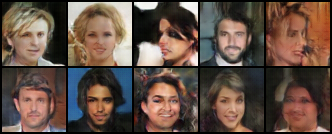
\includegraphics[width=0.84\textwidth]{generated_grid.png}
\caption{DCGAN 在 $64\times64$ 配置下的随机采样生成结果。该图由训练完成后的生成器在不同随机潜变量输入下得到，用于展示模型在标准采样模式下的人脸生成质量。}
\label{fig:dcgan-generated-grid}
\end{figure}

图 \ref{fig:dcgan-generated-grid} 展示了当前 DCGAN 模型在 $64\times64$ 分辨率下的随机采样结果。可以观察到，生成样本已经能够形成较稳定的人脸整体轮廓，并在发型、肤色、朝向以及背景亮度等因素上呈现一定多样性。多数样本的五官分布基本符合人脸拓扑结构，说明生成器已经学习到 CelebA 数据集中的主要外观模式。从视觉上看，图像的全局语义一致性优于训练初期常见的色块噪声状态，表明模型在对抗训练过程中逐步形成了较为合理的分布拟合能力。

与此同时，受限于原始 DCGAN 架构及 $64\times64$ 的输出分辨率，当前生成结果在局部纹理细节、边缘锐度和眼鼻口区域的精细建模方面仍存在明显局限。部分样本在发丝边缘、面部阴影和背景过渡区域仍可观察到模糊现象。这一结果与 DCGAN 的经典特性是一致的：其能够较好地捕获低分辨率下的人脸全局结构，但在更高频纹理恢复上仍受网络容量和训练稳定性制约。因此，在本次实验中，我们将 $64\times64$ 配置作为最终展示结果，是因为该分辨率下模型训练更稳定、样本观感也更均衡。

\subsubsection{线性插值实验}

\begin{figure}[H]
\centering

\includegraphics[width=0.88\textwidth]{interpolation_grid.png}
\caption{DCGAN 潜空间线性插值实验结果。图中展示了从随机潜变量 $z_1$ 平滑过渡到 $z_2$ 的生成样本变化过程。}
\label{fig:dcgan-interpolation}
\end{figure}

为进一步分析生成器是否学得连续且具有语义组织能力的潜空间表示，我们设计了潜变量线性插值实验。当前项目中的插值脚本并非在两张真实图像之间直接插值，而是首先随机采样两个潜变量 $z_1$ 与 $z_2$，然后在潜空间中按线性路径生成一系列中间点，并将这些中间潜变量送入生成器进行采样。图 \ref{fig:dcgan-interpolation} 给出了相应结果。

从插值结果可以看出，相邻样本之间的人脸姿态、头发轮廓、肤色亮度以及背景色块变化整体较为平滑，未出现大幅度的结构突变。这表明生成器学习到的潜空间并非离散孤立点集合，而具有一定连续流形特征。虽然个别过渡位置仍可见轻微模糊或语义不够稳定的现象，但整体上，插值路径能够保持基本的人脸可辨识性。这说明当前 DCGAN 模型在低分辨率设置下已经具备一定的潜表示组织能力，且未表现出严重的模式崩塌。

\subsubsection{定量评估结果}

\begin{table}[H]
\centering
\caption{DCGAN 在评估集上的 FID 与 IS 结果}
\label{tab:dcgan-metrics}
\begin{tabular}{ccc}
\toprule
Epoch & FID & IS \\
\midrule
5  & 23.3082 & 1.0404 \\
10 & 18.7192 & 1.0413 \\
15 & 15.0381 & 1.0438 \\
20 & 14.6819 & 1.0434 \\
25 & 14.8457 & 1.0447 \\
\bottomrule
\end{tabular}
\end{table}

在定量评估方面，我们采用 FID 和 IS 对生成结果进行联合分析，结果如表 \ref{tab:dcgan-metrics} 所示。FID 主要反映生成样本分布与真实样本分布的接近程度，因此其数值越低越好；IS 反映生成图像的可辨识性与多样性，因此其数值越高越好。由于两类指标关注的维度不同，单独依赖其中任意一项都可能造成误判。例如，较低的 FID 并不必然意味着局部纹理最优，较高的 IS 也不必然意味着生成分布完整覆盖了真实数据模式。

从表中可以看到，FID 从第 5 个 epoch 的 23.3082 持续下降至第 20 个 epoch 的 14.6819，说明生成分布与真实分布之间的距离在训练过程中显著缩小。到第 25 个 epoch 时，FID 略微回升到 14.8457，表明模型在后期已经接近局部稳定状态，继续训练带来的收益有限。相比之下，IS 从 1.0404 仅缓慢提升到 1.0447，整体增幅较小。这说明虽然模型在分布逼近方面有较明显改善，但在低分辨率设定下，样本的类别可辨识性与多样性提升并不显著。综合两项指标可认为：当前实现已经较好学习到人脸图像的主要统计结构，但在纹理精细度和视觉丰富性方面仍然存在改进空间。

\subsection{CycleGAN实验结果}
\subsubsection{风格迁移效果展示与分析}
\begin{figure}[H]
\centering

\includegraphics[width=0.92\textwidth]{picture1.png}\\[4pt]

\includegraphics[width=0.92\textwidth]{picture2.png}\\[4pt]

\includegraphics[width=0.92\textwidth]{picture3.png}
\caption{CycleGAN 在测试集上的真人头像到动漫头像风格迁移结果。每一行从左到右依次为 \texttt{real\_A}、\texttt{fake\_B}、\texttt{recov\_A} 与 \texttt{id\_A}，分别表示真人输入、迁移后的动漫头像、循环重建结果以及身份映射结果。}
\label{fig:cyclegan-qualitative}
\end{figure}

图 \ref{fig:cyclegan-qualitative} 给出了 CycleGAN 在测试集上的代表性可视化结果。第二列 \verb|fake_B| 显示，模型已经能够将真人头像稳定映射到动漫风格域：面部轮廓被保留的同时，肤色、眼部描边、发色块和背景色调均呈现出更明显的二次元风格特征。这说明生成器 $G_{AB}$ 已经学习到从真人头像统计分布到动漫头像统计分布的基本映射规律。

不过，从局部细节看，当前模型生成结果仍存在一定局限。部分样本在发丝边缘、脸部阴影过渡和眼口区域出现平滑化现象，说明动漫风格虽然能够被迁移，但纹理清晰度与边缘锐度仍不足。此外，不同样本间风格迁移强度并不完全一致：某些样本能够形成较强的卡通化特征，而另一些样本则更接近“带有动漫色彩的人脸照片”。这表明当前模型已经具备基础风格翻译能力，但其风格强度与局部细节建模仍有提升空间。

\subsubsection{循环一致性验证}
\verb|recov_A| 列反映了循环一致性约束的效果，即将真人头像先映射到动漫域，再映射回真人域后，是否仍能保持原有结构。从图 \ref{fig:cyclegan-qualitative} 可以看出，重建结果整体上保留了姿态、头部位置和大体五官布局，说明循环一致性损失确实在抑制大幅度结构崩塌方面发挥了作用。与此同时，\verb|id_A| 列展示了将真人样本直接送入 $G_{BA}$ 后的输出，用于衡量身份映射约束。若该列与 \verb|real_A| 差异过大，则说明模型会对已经位于目标域附近的样本做出过度修改。

从当前结果看，\verb|recov_A| 相较于 \verb|real_A| 仍然存在面部泛红、局部模糊和轻微几何扭曲现象，说明循环约束虽有效，但尚不足以完全保持内容信息。这与定量评估中偏高的循环重建误差是一致的。相较之下，\verb|id_A| 样本通常保留了基本头像结构，但在肤色、发色与背景区域仍可见不必要变化，说明身份映射损失已经能够起到正则化作用，但其约束强度仍不够充分。

\subsubsection{定量评估结果}
\begin{table}[H]
\centering
\caption{CycleGAN 在完整测试集上的定量评估结果}
\label{tab:cyclegan-metrics}
\begin{tabular}{cccc}
\toprule
$FID_{A2B}$ & $FID_{B2A}$ & $cycle\_L1_A$ & $cycle\_L1_B$ \\
\midrule
293.31 & 402.12 & 0.1089 & 0.0942 \\
\bottomrule
\end{tabular}
\end{table}

表 \ref{tab:cyclegan-metrics} 汇总了当前 CycleGAN 模型在整个测试集上的双向 FID 和循环重建误差。$FID_{A2B}$ 衡量真人头像经 $G_{AB}$ 迁移到动漫域后与真实动漫测试集之间的分布距离，$FID_{B2A}$ 则衡量反向迁移质量；两个指标越低越好。结果显示，$FID_{A2B}=293.31$，$FID_{B2A}=402.12$，说明正向迁移明显优于反向迁移，模型在动漫头像到真人头像的还原任务上更难学习到稳定分布。

循环重建方面，$cycle\_L1_A=0.1089$，$cycle\_L1_B=0.0942$，表明双向循环一致性都尚未达到较强约束水平。结合可视化结果可以推断：模型已经学会了“向目标域风格靠近”的基本方向，但在保留身份、精细结构与纹理细节方面仍存在明显误差。因此，当前 CycleGAN 结果更适合被理解为“已具备基础风格迁移能力，但尚未达到高保真跨域翻译”的实验阶段输出。

\subsection{两种模型对比分析}

\begin{table}[H]
\centering
\caption{DCGAN 与 CycleGAN 在任务目标与训练方式上的差异}
\label{tab:model-compare}
\begin{tabular}{>{\centering\arraybackslash}m{2.2cm} >{\centering\arraybackslash}m{3.2cm} >{\centering\arraybackslash}m{3.1cm} >{\centering\arraybackslash}m{4.8cm}}
\toprule
模型 & 输入形式 & 输出目标 & 主要评估方式 \\
\midrule
DCGAN & 随机潜变量 $z$ & 从零生成真人头像 & FID、IS、潜空间插值 \\
CycleGAN & 真人/动漫真实图像 & 真人头像与动漫头像之间的双向迁移 & $FID_{A2B}$、$FID_{B2A}$、循环重建误差、可视化对比 \\
\bottomrule
\end{tabular}
\end{table}

从任务属性上看，DCGAN 与 CycleGAN 虽同属对抗生成框架，但研究重点明显不同。DCGAN 面向“从噪声到图像”的无条件生成，其核心在于学习真实人脸分布，并考察潜空间组织能力，因此更关注生成样本的整体真实性、分布覆盖程度以及不同随机潜变量之间的语义连续性。CycleGAN 则面向“从一个图像域到另一个图像域”的无配对翻译任务，其关键不只是生成目标域风格，更在于在风格迁移过程中保留源图像的姿态、布局和身份相关结构，因此必须同时考察对抗质量和内容保持能力。

从实验结果上看，DCGAN 在 $64\times64$ 低分辨率场景下已经可以生成稳定的人脸整体结构，且 FID 指标随训练推进明显下降，说明其在低维生成任务中具有较好的可控性和稳定性。相比之下，CycleGAN 的任务难度更高：一方面需要在真人域与动漫域之间建立跨风格映射，另一方面还需要保持内容一致，因此当前实验虽然实现了基础风格迁移，但在反向映射质量、双向性能平衡和纹理细节保真度方面仍落后于理想状态。这也说明，风格迁移问题相较于低分辨率无条件生成，需要更强的结构约束、更充分的数据覆盖以及更稳健的训练策略。

\section{问题与改进}
\subsection{训练中遇到的问题及解决方法}
\paragraph{(1) DCGAN 的分辨率与清晰度矛盾}
在 DCGAN 实验中，$128\times128$ 配置虽然在结构上得到支持，但从实际训练结果看，其样本质量并未显著优于 $64\times64$ 配置，反而更容易出现模糊和训练不稳定问题。为保证最终报告中的展示效果，我们保留了 $64\times64$ 的生成结果作为主结果图，并将 $128\times128$ 视为结构扩展而非最终展示配置。这一现象说明，对于经典 DCGAN 而言，仅提高输出分辨率并不足以保证细节质量同步提升，还需要更强的模型容量与更长的稳定训练过程。

\paragraph{(2) CycleGAN 的学习率调度与训练轮数设置}
在 CycleGAN 的早期实验中，若学习率过大或训练轮数不足，模型容易表现为欠拟合：生成结果仍然保留大量源域纹理，动漫化程度不足，或者在训练后期波动较大。针对这一问题，当前实现采用了更符合原始 CycleGAN 经验设置的训练策略，即总训练 200 个 epoch，并从第 100 个 epoch 起线性衰减学习率。该策略使模型在前期充分学习跨域映射，在后期逐渐收敛，从而提升了训练稳定性。

\paragraph{(3) 对抗训练震荡与谱归一化}
在风格迁移实验中，双向 FID 值一度较高，且反向迁移性能弱于正向迁移。结合训练日志与可视化结果分析，这类问题通常与判别器过强、梯度震荡以及双域分布差异过大有关。当前实现为生成器和判别器卷积层都引入了谱归一化，其目的在于约束权重矩阵的谱范数，减弱训练过程中参数更新的不稳定性。实验现象表明，谱归一化确实有助于缓解明显的训练发散，但并未从根本上消除双向性能不均衡的问题。

\subsection{模型局限性与改进方向}
\paragraph{(1) DCGAN 的局限性}
当前 DCGAN 模型的主要局限体现在分辨率和纹理表达能力上。尽管其在 $64\times64$ 分辨率下可以较好学习人脸整体结构，但对于头发边缘、眼口局部纹理和背景过渡的高频细节建模仍较薄弱。后续若要进一步提升人脸生成质量，可以从两方面改进：一是引入更强的多尺度生成架构，如渐进式增长或风格调制网络；二是结合更加稳定的对抗训练策略，如改进损失函数或引入感知约束。

\paragraph{(2) CycleGAN 的局限性}
CycleGAN 当前最明显的问题是双向性能不均衡与循环一致性不足。正向真人到动漫迁移已经具备可见效果，但反向动漫到真人的 FID 显著更高，说明目标域分布拟合仍然不足。同时，循环重建误差偏高，表明模型在风格迁移过程中会损失一定内容信息，导致面部结构、肤色和发色出现偏移。对于这类问题，后续可以尝试提高循环一致性或身份映射损失权重，引入感知损失以强化内容保持，并通过更细致的数据筛选和分阶段微调减小双域统计差异。

\paragraph{(3) 面向后续工作的整体思路}
从本次实验可以看出，无条件人脸生成与无配对风格迁移虽然都属于 GAN 应用，但其优化重点并不相同。前者更依赖分布学习和潜空间表达，后者更强调结构保持与域间映射稳定性。因此，后续工作若继续围绕人头图像生成展开，可以考虑将两类方法结合：例如，先通过更强的生成模型获得质量更高的真人头像，再引入结构约束更强的风格迁移模型进行二次转换，从而实现兼顾真实性、风格性与可控性的完整头像生成流程。

\section{总结}

我们围绕基于 GAN 的人头图像生成与风格迁移任务，分别实现并分析了 DCGAN 与 CycleGAN 两类代表性模型。对于 DCGAN，我们完成了面向 CelebA 数据集的单卡 GPU 训练系统，实现了 $64\times64$ 与 $128\times128$ 双结构支持、训练/评估集划分、随机采样、潜空间线性插值以及 FID/IS 评价。实验结果表明，该模型在 $64\times64$ 分辨率下能够生成具有基本人脸结构的样本，且潜空间具有较好的连续性，但在细节纹理和高分辨率稳定生成方面仍存在不足。

对于 CycleGAN，我们基于标准 \texttt{trainA/trainB/testA/testB} 数据组织完成了真人头像与动漫头像之间的无配对风格迁移实验，实现了双向生成器、双向判别器、循环一致性和身份映射约束，以及面向完整测试集的双向 FID 与重建误差评估。实验表明，该模型已经能够完成基础风格迁移，尤其在真人头像到动漫头像方向上具有较明确的风格转换效果；但与此同时，反向映射质量、双向性能平衡与高保真内容保持仍是当前实现的主要瓶颈。

总体而言，我们的工作较为系统地复现并比较了两类经典 GAN 模型在头像生成任务中的行为特点：DCGAN 更适合研究从噪声到图像的分布建模与潜空间表达，而 CycleGAN 更适合研究无配对跨域映射中的结构保持与风格控制。通过对二者的实现、实验与结果分析，可以更清晰地理解对抗生成模型在不同视觉任务中的建模重点及其工程挑战。

\section{参考文献}
\begin{thebibliography}{99}
\bibitem{goodfellow2014gan}
Goodfellow I, Pouget-Abadie J, Mirza M, et al.
Generative Adversarial Nets[C]//Advances in Neural Information Processing Systems.
2014: 2672--2680.

\bibitem{radford2015dcgan}
Radford A, Metz L, Chintala S.
Unsupervised Representation Learning with Deep Convolutional Generative Adversarial Networks[EB/OL].
\url{https://arxiv.org/abs/1511.06434}, 2015.

\bibitem{salimans2016improved}
Salimans T, Goodfellow I, Zaremba W, et al.
Improved Techniques for Training GANs[EB/OL].
\url{https://arxiv.org/abs/1606.03498}, 2016.

\bibitem{heusel2017fid}
Heusel M, Ramsauer H, Unterthiner T, et al.
GANs Trained by a Two Time-Scale Update Rule Converge to a Local Nash Equilibrium[C]//Advances in Neural Information Processing Systems.
2017: 6626--6637.

\bibitem{liu2015celeba}
Liu Z, Luo P, Wang X, Tang X.
Deep Learning Face Attributes in the Wild[C]//Proceedings of the IEEE International Conference on Computer Vision.
2015: 3730--3738.

\bibitem{zhu2017cyclegan}
Zhu J Y, Park T, Isola P, Efros A A.
Unpaired Image-to-Image Translation using Cycle-Consistent Adversarial Networks[C]//Proceedings of the IEEE International Conference on Computer Vision.
2017: 2223--2232.

\bibitem{johnson2016perceptual}
Johnson J, Alahi A, Fei-Fei L.
Perceptual Losses for Real-Time Style Transfer and Super-Resolution[C]//Proceedings of the European Conference on Computer Vision.
2016: 694--711.
\end{thebibliography}

\section{附录}
\subsection{DCGAN核心代码}

附录仅保留与当前实现直接相关的核心代码片段，用于说明网络结构、数据划分、训练过程与评估入口。

\lstinputlisting[
    caption={DCGAN 双分辨率生成器与判别器结构（取自 \texttt{dcgan\_model.py}）},
    label={lst:dcgan-model},
    firstline=7,
    lastline=88
]{../DCGAN/dcgan_model.py}

\lstinputlisting[
    caption={DCGAN 训练集/评估集划分逻辑（取自 \texttt{main.py}）},
    label={lst:dcgan-split},
    firstline=153,
    lastline=198
]{../DCGAN/main.py}

\lstinputlisting[
    caption={DCGAN 训练主循环中的判别器与生成器更新（取自 \texttt{main.py}）},
    label={lst:dcgan-train-loop},
    firstline=377,
    lastline=405
]{../DCGAN/main.py}

\lstinputlisting[
    caption={DCGAN 评估入口与按 epoch 记录 FID/IS（取自 \texttt{main.py}）},
    label={lst:dcgan-eval},
    firstline=354,
    lastline=368
]{../DCGAN/main.py}

\subsection{CycleGAN核心代码}

\lstinputlisting[
    caption={CycleGAN 残差块、生成器与 PatchGAN 判别器（取自 \texttt{models.py}）},
    label={lst:cyclegan-models},
    firstline=23,
    lastline=123
]{../cycle-GAN2/models.py}

\lstinputlisting[
    caption={CycleGAN 训练中的总损失计算（取自 \texttt{cyclegan.py}）},
    label={lst:cyclegan-loss},
    firstline=222,
    lastline=253
]{../cycle-GAN2/cyclegan.py}

\lstinputlisting[
    caption={CycleGAN 训练时的八图可视化逻辑（取自 \texttt{cyclegan.py}）},
    label={lst:cyclegan-sample},
    firstline=175,
    lastline=199
]{../cycle-GAN2/cyclegan.py}

\lstinputlisting[
    caption={CycleGAN 基于完整测试集的双向评估逻辑（取自 \texttt{evaluate.py}）},
    label={lst:cyclegan-eval},
    firstline=92,
    lastline=165
]{../cycle-GAN2/evaluate.py}

\end{document}
